\documentclass[12pt,relax]{TrilinosOverview}

\title{An Overview of the Trilinos Project}
\SANDsubtitle{}

\author{Michael A.~Heroux, Roscoe Bartlett, David Day, \\
Robert Hoekstra, Jonathan Hu, Tamara Kolda, \\
Rich Lehoucq, Kevin Long, Roger Pawlowski, \\
Andrew Rothfuss, Andrew Salinger, Heidi Thornquist, \\
Ray Tuminaro, Jim Willenbring, Alan Williams \\
 \\
Sandia National Laboratories\\
P.O. Box 5800\\
Albuquerque, NM 87185-1110 \\
maherou@sandia.gov
}

\date{}


\SANDnum{SAND2003-xxxx}
\SANDprintDate{June 2003}
\SANDauthor{
Michael A.~Heroux, Roscoe Bartlett, David Day, \\
Robert Hoekstra, Jonathan Hu, Tamara Kolda, \\
Rich Lehoucq, Kevin Long, Roger Pawlowski, \\
Andrew Rothfuss, Andrew Salinger, Heidi Thornquist, \\
Ray Tuminaro, Jim Willenbring, Alan Williams \\
 \\
Sandia National Laboratories}


\SANDreleaseType{Unlimited Release}


\SANDdistcategory{UC-999}


\begin{document}
\maketitle

\begin{abstract}
The Trilinos Project is an effort to facilitate the design,
development, integration and ongoing support of mathematical software
libraries.  In particular, our goal is to develop parallel solver 
algorithms and libraries within 
an object-oriented software framework for the solution of large-scale, complex
multi-physics engineering and scientific applications.   Our emphasis is on 
developing robust, scalable algorithms in a software framework, using abstract 
interfaces for flexible interoperability of components and providing a 
full-featured set of concrete classes that implement all abstract
interfaces.  

Trilinos uses a two-level software structure designed around
collections of a
{\it packages}.  A Trilinos package is an integral unit usually
developed by a small team of experts in a particular algorithms area
such as algebraic preconditioners, nonlinear solvers, etc.

Trilinos components are primarily written in C++, but provide essential C and 
Fortran user interface support.  We provide an open architecture that allows 
easy integration with other solver packages and we deliver our software to 
the outside community via the Gnu Lesser General Public License
(LGPL)~\cite{gnu-license-site}.
This report provides an overview of Trilinos, discussing the 
objectives, history, current development and future plans of the project.
\end{abstract}


\clearpage
\section*{Acknowledgement}
The authors would like to acknowledge the support of the ASCI and LDRD programs
that funded development of Trilinos.



\clearpage
\tableofcontents
\listoffigures
\listoftables


\clearpage
\section{Summary}

A core requirement of many engineering and scientific applications is 
the need to solve linear and non-linear systems of equations, eigensystems 
and other related problems.  Thus it is no surprise that any 
part of the application that solves these problems is called a ``solver.'' 
The exact definition of what specifically constitutes a solver depends on 
many factors.  However, a good working definition of a solver is
the following: {\it Any piece of software that finds unknown values for 
some set of discrete governing equations in 
an application.}  Another characteristic of solvers is that we can often 
implement them in such a way that they are ``general-purpose'', so that the
details of how the discrete problem was formed are not specifically needed 
for the solver to work (although information about problem characteristics 
can often be vital to robust solutions.)

General-purpose linear and eigensolvers have been successfully used across 
a broad set of applications and computer systems.  EISPACK~\cite{eispack}, 
LINPACK~\cite{linpack} and LAPACK~\cite{lapack} are just a few of
the many packages that have made a tremendous impact, providing robust 
portable solvers to a broad set of applications.  More recently packages 
such as PETSc~\cite{petsc-home-page,petsc-manual,petsc-efficient} 
and Aztec~\cite{Aztec2.1} have provided a large
benefit to applications by giving users access to parallel distributed 
memory solvers that are easy-to-use and robust.

Sandia has historically had efforts to develop scalable solver algorithms 
and software.  Often this development has been done within the context of 
a specific application code, providing a good robust solver that 
specifically meets the needs of that application.  Even Aztec, one of 
the most important general-purpose solvers developed at Sandia, was 
developed specifically for MPSalsa~\cite{MPSalsa-User-Guide,MPSalsa-Theory} 
and only later extracted for use with other applications.  Unfortunately, 
even though application-focused solvers tend to be very robust and can 
often be made into very effective general-purpose solvers, the 
opportunity to re-use the basic set of tools developed for one solver 
in the development of another solver becomes very difficult.

The Trilinos Project grew out of this group of established numerical algorithms
efforts at Sandia, motivated by  a recognition that a modest degree of 
coordination among these efforts could have a large positive impact on 
the quality and usability of the software we produce and therefore enhance the
research, development and integration of new solver algorithms into
applications.  Although the project has existed for only two years, 
the degree of effort required to develop new parallel solvers has been 
substantially reduced because our common infrastructure provides an excellent 
starting point.  Furthermore, many applications are standardizing on the 
Trilinos matrix and vector classes.  As a result, these applications
have access to all Trilinos solver components without any unnecessary 
interface modifications.

This document provides an overview of the Trilinos project,
focusing on the project philosophy and description, and
providing the reader with an summary of the project in its current state.  


\clearpage
\section*{Nomenclature}
\addcontentsline{toc}{section}{Nomenclature}
\begin{itemize}
\item[Package]
A collection of software focused on one primary class of numerical
methods.  Also a fundamental, integral unit in the Trilinos framework.

\item[Trilinos]
The name of the project.  Also a Greek term which,
loosely translated means ``a string of pearls,'' 
meant to evoke an image that each Trilinos package is a pearl in its 
own right, but is even more valuable when combined with other 
packages.

\item[new\_package] A sample Trilinos package containing all of the
infrastructure to install a new package into the Trilinos framework.
Contains the basic directory structure, a collection of sample
configuration and build files and a sample ``Hello World'' package.

\item[Anasazi]
An extensible and interoperable framework for large-scale eigenvalue
algorithms.The motivation for this framework is to provide a generic
interface to a collection of algorithms for solving large-scale 
eigenvalue problems.

\item[AztecOO] 
Linear solver package based on preconditioned Krylov methods.  A 
follow-on to the Aztec solver package~\cite{Aztec2.1}.  
Supports all Aztec 
interfaces and functionality, but also provides significant new 
functionality.

\item[Belos] A Greek term meaning ``arrow.'' Belos is the next
generation of iterative solvers.  Belos solvers are written using
``generic'' programming techniques.  In other words, Belos is written
using TSF abstract interfaces and therefore has no explicit dependence
on any concrete linear algebra library.  Instead, Belos solvers can be
used with any concrete linear algebra library that implements the TSF
abstract interfaces. 

\item[Ifpack] 
Object-oriented algebraic preconditioner, compatible with 
Epetra and AztecOO.  Supports construction and use of parallel
distributed memory preconditioners such as overlapping Schwarz domain
decomposition, Jacobi scaling and local Gauss-Seidel relaxations.

\item[Komplex] 
Complex linear equation solver using equivalent real 
formulations~\cite{DayHero2000}, built on top of Epetra and AztecOO.

\item[Meros]
Segregated preconditioning package.  Provides scalable block
preconditioning for problems that couple simultaneous solution
variables such as Navier-Stokes problems.

\item[ML]
Algebraic multi-level preconditioner package.  Provides scalable
preconditioning capabilities for a variety of problem classes.

\item[NOX]
A collection of nonlinear solvers, designed to be easily integrated
into an application and used with many different linear solvers.

\item[Petra]
A Greek term meaning ``foundation.''  Trilinos has three Petra 
libraries: Epetra, Tpetra and Jpetra that provide basic classes 
for constructing and manipulating matrix, graph and vector
objects.  Epetra is the current production version that is
split into two packages, one core and one extensions.

\begin{itemize}

\item[Epetra] Current C++ production implementation of the Petra
Object Model.  The ``E'' in Epetra stands for ``essential'' implying
that this version provides the most important capabilities that are
commonly needed by our target application base.  Epetra supports real,
double-precision floating point data only (no single-precision or
complex).  Epetra avoids explicit use of some of the more
advanced features of C++, including templates and the Standard
Template Library, that can be impediments to portability.

\item[Tpetra] The future C++ version of Petra, using templates and
other more advanced features of C++.  Tpetra supports arbitrary scalar
and ordinal types, and makes extensive use of advanced C++ features.

\item[Jpetra] A Java implementation of Petra, supporting real,
double-precision data.  Written in pure Java, it is designed to be
byte-code portable and can be executed across multiple compute nodes.

\end{itemize}

\item[Teuchos] A collection of classes and service software that is
useful to almost almost all Trilinos packages.  Includes
reference-counted pointers, parameter lists, templated interfaces to
BLAS, LAPACK and traits for templates.  

\item[TSF] A collection of abstract interfaces that supports application
access to a variety of Trilinos capabilities, supports
interoperability betweeen Trilinos packages and provides future extensibility.
TSF is composed of several packages.  The primary user packages are:  
\begin{itemize}

\item[TSFCore] TSFCore provides 
a basic collection of abstract interfaces to vectors, linear
operators, solvers, etc.  These interfaces provide a common
interface for applications to access one or more packages that
implement the abstract interface.  These interfaces can also be used
by other packages in Trilinos to accomplish the same purpose.

\item[TSFExtended] TSFExtended builds on top of TSFCore, providing implicit
aggregation capabilities and overloaded operators.  
\end{itemize}

\end{itemize}


\section{Introduction}

Research efforts in advanced solution algorithms and parallel solver
libraries have historically had a large impact on engineering and
scientific computing.  Algorithmic advances increase the range
of tractable problems and reduce the cost of solving existing
problems.  Well-designed solver libraries provide a mechanism for
leveraging solver development across a broad set of applications and
minimize the cost of solver integration.  Emphasis is
required in both new algorithms and new software in order
to achieve the maximum impact of efforts.

The Trilinos project encompasses a variety of efforts that are to some
extent self-contained but at the same time inter-related.  The
Trilinos design allows individual packages to grow and mature
autonomously to the extent the algorithms and package developers
dictate. 

Integration of a package into Trilinos, and what Trilinos can provide
to a package, have multiple possibilities
that will be discussed in Section~\ref{sect:TrilinosDesign}.
Section~\ref{sect:PetraAndTSF} discusses two special Trilinos
packages: Epetra and TSF.  The general definition of a Trilinos
package is presented in Section~\ref{sect:PackageDefinition}
An overview of current software research and
development is given in Section~\ref{sect:Software}.  
Finally, this document contains
an Appendix~\ref{sect:OOTutorial} which gives a brief
tutorial on object-oriented concepts for readers who are unfamiliar
with the area.  

\section{Trilinos Design Philosophy}
\label{sect:TrilinosDesign}
Each Trilinos package is a self-contained, independent piece
of software with its own set of requirements, its own development team
and group of users.  Because of this,
Trilinos itself is designed to respect the autonomy of packages.
Trilinos offers a variety of ways for a particular package to interact 
with other Trilinos packages.  It also offers a set of tools that can
assist package developers with builds across multiple platforms, generating
documentation and regression testing across a set of target platforms.
At the same time, what a package {\it must} do to be called a Trilinos
package is minimal, and varies with each package.  The current
collection of Trilinos packages is shown in Figure~\ref{Figure:TrilinosPackages}.

\begin{figure}
\begin{center}
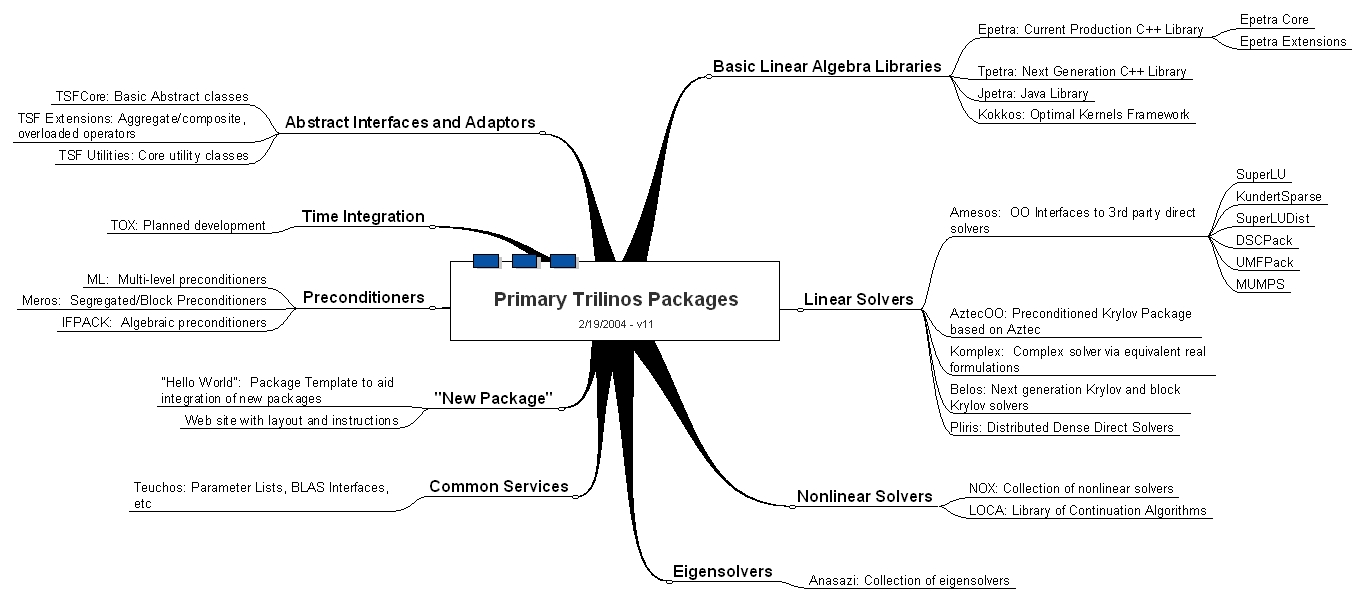
\includegraphics[height=9in]{../CommonFiles/TrilinosPackagesDiagram}
\end{center}
\label{Figure:TrilinosPackages}
\caption{Current collection of Trilinos Packages}
\end{figure}

\subsection{Services Provided by Trilinos}

Trilinos provides a variety of services to a developer wanting to
integrate a package into Trilinos.  In particular, the following are
provided:
\begin{itemize}
\item Configuration management:
Autoconf~\cite{Autoconf},  Automake~\cite{Automake} and
Libtool~\cite{Libtool} provide a robust, full-featured set of tools for
building software across a broad set of platforms (see also the ``Goat
Book''~\cite{GoatBook}).  Although these
tools are not official standards, they are commonly used in many
packages.  Nearly all existing
Trilinos packages use Autoconf and Automake.  Libtool support will be
added in future releases. 

Package developers who are not currently using autotools, but would like
to, can get a jump start by using a Trilinos package called
``new\_package''.  This trivial package exists for one primary purpose.
It walks a developer through the process of setting up a package to
configure and build using autotools.  This package is not yet complete, 
but is far enough along to be of use to a developer who does not have 
extensive Autotools experience. 
 

Trilinos provides a set of M4~\cite{M4} macros that can be used by any other
package that wants to use Autoconf and Automake for configuring and
building libraries.  These macros perform common configuration tasks such as
locating a valid LAPACK~\cite{lapack} library, or checking for a user-
defined MPI C compiler.  These macros minimize the amount of redudant
 effort in using Autotools, and make it easier to apply a general change to
the configure process for all packages.  However, use of these tools is not 
required.


\item Regression testing: Trilinos provides a variety of regression
testing capabilities.  Although the test suite is always improving,
good coverage testing is available for the major Trilinos packages.
Integrating new tests into Trilinos is accomplished by creating
specially named directories in the CVS repository and creating scripts
that run package tests.  These scripts can be executed manually and
are also run as part of the automated regression test harness (see
next item).

\item Periodic Testing: Trilinos Packages that configure and build using 
Autotools can easily utilize the the Trilinos test harness.  On a nightly 
basis, the test harness builds the most recent versions of Trilinos libraries 
and runs any tests that have been integrated into the testharness.  Currently 
the testharness only runs on Linux, IRIX64, and DEC/OSF1, but it will 
eventually run on 5-8 platforms.

\item Portable interface to BLAS and LAPACK: The Basic Linear Algebra
Subprograms (BLAS)~\cite{BLAS1,BLAS2,BLAS3} and LAPACK~\cite{lapack}
provide a large repository of robust, high-performance mathematical
software for serial and shared memory parallel dense linear algebra
computations.  However, the BLAS and LAPACK interfaces are Fortran
specifications, and the mechanism for calling Fortran interfaces from
C and C++ varies across computing platforms.  Epetra (and Teuchos)
provide a set of simple, portable interfaces to the BLAS and LAPACK
that provide uniform access to the BLAS and LAPACK across a broad
set of platforms.  These interfaces are accessible to
other packages.

\item Source code repository and other software process tools:
Trilinos source code is
maintained in a CVS~\cite{CVS} repository that is accessible via a
secure connection from anywhere on the internet.  It is also browsable
via a web-based interface package called Bonsai~\cite{Bonsai}.  Features 
and bug reports are tracked using Bugzilla~\cite{Bugzilla}, and email 
lists are
maintained for Trilinos as a whole and for each package.  Support for new
packages can easily be added.  All tools are accessible from the main
Trilinos website~\cite{Trilinos-home-page}.

\item Quick-start package infrastructure: Via the new\_package package in
Trilinos, a new or existing software project can quickly adopt a
variety of useful software processes and tools.  new\_package provides a
starting point for:
\begin{itemize}
\item Project organization:  Illustrates one way of
organizing files for a mathematical software package.
\item Autotools: As mentioned above, provides simple working example
using autotools, and a set of M4 macros.
\item Automatically generated reference documentation: Shows how
to mark up source code and use Doxygen~\cite{Doxygen} to produce
accurate, extensive source code documentation.
\item Regression testing: Simple regression testing example is part of
new\_package.
\item Website: The Trilinos home page~\cite{Trilinos-home-page}
contains a new\_package website that includes instruction on how to
copy and modify the new\_package web source for use with a new
Trilinos package.
\end{itemize}

It is worth noting that the Trilinos new\_package package can be
useful independent of Trilinos itself.  Like all Trilinos packages,
new\_package is self-contained, and can be configured and
built independently from the rest of Trilinos.  Similarly, the
new\_package website is self-contained and essentially independent
from the rest of the Trilinos website.
\end{itemize}

\section{Petra and TSF: Two Special Package Collections}
\label{sect:PetraAndTSF}
In order to understand what Trilinos provides beyond the
contributions of each Trilinos package, we briefly discuss two special
collections of
Trilinos packages: Petra and TSF.  These two packages collections are
complimentary, with TSF packages providing common abstract application
programmer interfaces (APIs) for other Trilinos packages and Petra
providing common concrete implementations of basic classes used by most
Trilinos packages.  Within the Petra collection of packages, Epetra is
the most mature, portable and widely used package.  Within the TSF
collection, TSFCore provides a lean set of interfaces and TSFExtended
provides a fuller feature set.  TSFExtended builds on top of TSFCore,
i.~e.~, TSFExtended classes inherit from TSFCore classes.

\subsection{Epetra}
Matrices, vectors and graphs are basic objects used in most solver
algorithms. Most Trilinos
packages interact with these kinds of objects via abstract interfaces that
allow a package to define what services and behaviors are expected from 
the objects,
without enforcing a specific implementation.  However, in order to use
these packages, some concrete
implementation must be selected.  Epetra (and in the future other 
packages described
in Section~\ref{subsect:PetraObjectModel}) is a collection of concrete
classes that supports the construction and use of vectors, sparse
graphs, and dense and sparse matrices.  It provides serial, parallel and
 distributed memory
capabilities.  It uses the BLAS and LAPACK where possible, and as a
result has good performance characteristics.

\subsection{TSFCore and TSFExtended}
\label{subsect:InteropTSF}
Many different algorithms are available to solve a given numerical
problem.  For example, there are many algorithms for solving a system
of linear equations, and many solver packages are available to solve
linear systems.  Which package is appropriate is a function of
many details about the problem being solved and the platform on which
application is being run. However, even though
there are many different solvers, conceptually, from an abstract view,
these solvers are providing a similar capability, and it is
advantageous to utilize this abstract view.
TSF is a collection of abstract classes that provides an application
programmer interface (API) to perform the most common solver
operations.  It can provide a single interface to many different
solvers.  Furthermore, TSFExtended has powerful compositional
mechanisms that support the
light-weight construction of composite objects from a set of
existing objects.  As a result, TSF users gain easy access to many
solvers and can bring multiple solvers to bear on a single problem.


\section{Trilinos Package Interoperability Mechanisms}
\label{sect:PackageDefinition}
As mentioned above, what a package {\it must} do to be called a Trilinos
package is minimal, and varies with each package.  In this section we
list the primary mechanisms for a package to become part of Trilinos.
Note that each mechanism is an extension or augmentation of package
capabilities, creating connections between packages.  Thus, a package does 
not need to change its internal structure to become part of Trilinos.

\subsection{Mechanism 1: Package Accepts User Data as Epetra Objects}
All solver packages require some user data (usually in the form of
vectors and matrices) or require the user to supply the action of an
operator on a vector.  Accepting this data in the form of Epetra
objects is the first Trilinos interoperability mechanism.  Any package
that accepts user data this way immediately becomes accessible to an
application that has built its data using Epetra.  We expect every
Trilinos package to implement this mechanism in some way.  Since
Epetra provides a variety of ways to extract data from an Epetra
object, minimally we expect that a package can at least copy data from
the user objects that were built using Epetra.  More often, a well-designed
package can typically encapsulate Epetra objects and ask for services from
the Epetra objects without explicitly copying them.  In the future, as
Tpetra matures (and C++ compilers mature), we expect Tpetra to be a
companion package to Epetra, fulfilling a similar role.

\subsection{Mechanism 2: Package Callable via TSF Interfaces}
TSF provides a set of abstract interfaces that can be used to
interface to a variety of solver packages.  TSF can accept
pre-constructed solver objects, e.g., preconditioners, iterative
solvers, etc., by simple encapsulation or it can
construct solver objects using one of a variety of factories.  (See
Appendix~\ref{sect:OOTutorial} for the definition of a factory.)  Once
constructed, a solver object can be further modified by passing it a
parameter list containing a list of key-value pairs that can control
solver behavior when it is trying to solve a problem.  For example,
the parameter list could specify a residual tolerance for an iterative solver.

A package is callable via TSF if it implements one or more of the TSF
abstract class interface, making it available to TSF users as one of a
suite of possible solver options.

\subsection{Mechanism 3: Package Can Use Epetra Internally}

Another interoperability mechanism available to a package is that of
using Epetra objects as the
internal objects for storing vector, matrices, etc. that are seldom or
never seen by the user.  In many instances, this mechanism has no
practical advantages.  However, in some instances, there can be a
saving in storage requirements.  Furthermore, by using Epetra objects
internally, a package can in turn use other Trilinos packages to
manipulate its own internal objects.

\subsection{Mechanism 4: Package access solver service via TSF interface}
TSF provides an abstract solver interface with access to multiple concrete 
solvers. 
A package can access solver services via TSF and therefore be able to use
any solver that implements the TSF interface.

\subsection{Mechanism 5: Package Builds Under Trilinos {\tt configure} Scripts}
Trilinos uses Autoconf~\cite{Autoconf} and Automake~\cite{Automake} to
build libraries and test suites.  The Trilinos directory structure
keeps each Trilinos package completely self-contained.  As such, each
package is free to use its own configuration and build process.  At
the same time, Trilinos has a top-level configure script that traverses
the directory structure invoking package configure scripts,
passing on any parameter definitions
from the top level.  Similarly, the make process is also recursive.

A package may easily be automatically built from the top-level
Trilinos configuration and make process by copying and modifying the
Autoconf and Automake scripts from another package.  The benefit for
doing this is that Autoconf and Automake improve the portability of a
package across a broad set of platforms.  Also, Automake provides a
rich set of targets for building libraries, software distributions,
test suites and installation processes.  If a package adopts the
Trilinos configuration and build process, it will be built
automatically along with a large number of other Trilinos packages.

\section{Overview of Current Package Development}
\label{sect:Software}

\subsection{The Petra Object Model}
\label{subsect:PetraObjectModel}
The Petra class libraries provide a
foundation for all Trilinos solver development.  Petra provides 
object classes for
constructing and using parallel, distributed memory matrices and vectors.  
Petra exists in
multiple forms.  Its most basic form is as an object 
model~\cite{HeroHoekWill2002}.
As such, it is an abstract 
description of a variety of vector, matrix and supporting classes, along with a 
description of
how these classes interact.  There are presently three implementations
of the Petra Object Model: Epetra, Tpetra and Jpetra.

\subsection{Epetra: Essential Implementation of Petra Object Model}

Epetra~\cite{Epetra-User-Guide}, the current production version of Petra,
 is written for real-valued double-precision scalar field data only, and
restricts itself to a stable core
of the C++ language standard.  As such, Epetra is very portable and 
stable, and  
is accessible to Fortran and C users.  
Epetra is unique in that it combines in a single package (i) support 
for generic parallel
machine descriptions, (ii) extensive use of standard numerical 
libraries, (iii) use of best
practices in object-oriented C++ programming and (iv) parallel data 
redistribution.
Other basic linear algebra packages, e.~.g.~ the Template Numerical 
Toolkit~\cite{TNT-site},
PETSc~\cite{petsc-manual} and the Matrix Template 
Library~\cite{SiekLums98}, feature one
or two of these aspects only.  The availability of Epetra has 
facilitated rapid development
of numerous applications and solvers at Sandia because many of the 
complicated issues of
working on a parallel distributed memory machine are handled by Epetra.

Application developers can use Epetra to construct and manipulate matrices
and vectors, and then pass these objects to most Trilinos solver components.
Furthermore, solver developers can develop many new algorithms relying 
solely on Epetra classes to handle the intricacies of parallel execution.  
Epetra also has extensive parallel data  redistribution capabilities, 
including an interface to the Zoltan load-balancing
library~\cite{zoltan-ug}.  Epetra is split into two packages:  a core
package and a set of extensions.

\subsection{Tpetra: Templated C++ Implementation of Petra Object Model}

In addition to Epetra, we have started development of a templated 
version of Petra, called Tpetra, that implements the scalar and 
ordinal fields as templated types.  When fully developed, Tpetra 
will allow matrices and vectors to be composed of real or complex, 
and single or double precision scalar values.  Furthermore, in 
principle, any abstract data type (ADT) can be used as the scalar 
field type as long as the ADT supports basic mathematical operations 
such as addition and multiplication and inversion. Specifically, we 
could compute using an interval scalar field, matrices, integers, etc., 
without any additional code development in Tpetra.  Tpetra can also 
use any size integer for indexing.  Typically the ordinal field would 
be an integral data type such as int or long int.  However, any ADT 
that supports an indexing capability can be used, including integers in 
other bases, or cyclic indexing. Additionally, Tpetra also uses the 
C++ language standard more fully.  In particular, it utilizes the 
Standard Template Library (STL)~\cite{Stroustrup}, to provide maximal 
algorithmic efficiency with minimal code development.

We will fully develop Tpetra as a peer library to Epetra. By using partial
specialization of templates, we will base Tpetra on established libraries 
such as the BLAS~\cite{BLAS1,BLAS2,BLAS3} and LAPACK~\cite{lapack} and 
therefore acquire the performance and robustness of these libraries.
Like Epetra, Tpetra is written for generic parallel distributed
memory computers whose nodes are
potentially shared memory multiprocessors.

\subsection{Jpetra: Java Implementation of Petra Object Model}

In addition to Tpetra, we have started a Java implementation of Petra.  
The primary design goals of this project are to produce a library that 
is a high performance, pure Java implementation of Petra.  By restricting 
ourselves to Java and avoiding the use of the Java Native Interface 
(JNI)~\cite{JNI-site} to link to other libraries, we get the true 
portability that Java promises.  The fundamental implication of these 
goals is that we cannot rely on BLAS~\cite{BLAS1,BLAS2,BLAS3}, 
LAPACK~\cite{lapack} or MPI~\cite{MPI} since they are not written in 
Java, and we do not use the JNI.  As such, we must track the development 
of pure Java equivalents of these libraries.  Several efforts, including 
Ninja~\cite{MoreMidkGuptArtiWuAlma2001} and 
MPJ~\cite{CarpGetoJuddSkjeFox2000}, provide equivalent functionality 
to the BLAS, LAPACK and MPI, but are completely written in Java.

We will fully implement Jpetra as a peer library to Epetra.  By making 
extensive use of Java interfaces, we can create loose dependencies on 
emerging BLAS, LAPACK and MPI replacements as they become mature and 
stable.  Recently, several research 
efforts~\cite{MoreMidkGuptArtiWuAlma2001,SCIMARK-site} have shown 
that there is no fundamental performance bottleneck using Java.  
Instead, Java compilers and user practices have been the issue.  
As a result, Java holds much promise as a high performance computing 
language.  Jpetra will facilitate adoption of Java in scientific and 
engineering applications.   Java also has native graphical user 
interfaces (GUI) support.  A significant part of Jpetra will be 
the development of GUI tools for visualization and manipulation of 
Jpetra objects.


\subsection{TSF: The Trilinos Abstract Class Packages}

Many different algorithms are available to solve any given numerical
problem.  For example, there are many algorithms for solving a system
of linear equations, and many solver packages are available to solve
linear systems.  Which package is appropriate is a function of
many details about the problem being solved and the platform on which
application is being run. However, even though
there are many different solvers, conceptually, from an abstract view,
these solvers are providing a similar capability, and it is
advantageous to utilize this abstract view.
TSF is a collection of abstract classes that provides an application
programmer interface (API) to perform the most common solver
operations.  It can provide a single interface to many different
solvers and has powerful compositional mechanisms that support the
light-weight construction of composite objects from a set of
existing objects.  As a result, TSF users gain easy access to many
solvers and can bring multiple solvers to bear on a single problem.

TSF is split into several packages.  The most important user-oriented
classes are TSFCore and TSFExtended:
\begin{enumerate}
\item {\bf TSFCore:} As its name implies, TSFCore contains a small set
of core classes that are considered essential to almost any abstract
linear algebra interface.  The primary user classes in TSFCore are
Vector, MultiVector, LinearOp and VectorSpace. TSFCore is discussed in
detail in~\cite{TSFCore}.
\item {\bf TSFExtended:} TSFExtended builds on top of TSFCore and
includes overloaded, block and composite operators, all of
which support powerful abstraction capabilities.  The Meros package
relies on TSFExtended to implicitly construct sophisticated
Schur compliment preconditioners in terms of exising component
operators with little overhead in time or memory.
\end{enumerate}

Both TSFCore and TSFExtended are important because they allow
interfacing and sophisticated use of numerical linear algebra objects
without requiring the user or application to commit to any particular
concrete linear algebra library.  This approach allows us to leverage
the investment in sophisticated abstract numerical algorithms across
many concrete linear algebra libraries and gives application
developers a single API that provides access to many solver packages.

TSF provides abstract interfaces for vector, matrix, operator and 
solver objects.  In addition, it has powerful aggregation mechanisms 
that allow existing TSF objects to be combined in a variety of ways 
to create new TSF objects.  TSF can be useful in many situations.  
For example:
\begin{enumerate}

\item Generic Krylov method implementation:  If a preconditioned Krylov solver 
is implemented using TSF vectors and operators, then any concrete package 
that implements the TSF vector and operator interfaces can be used 
with the Krylov solver.

\item Generic solver driver:  If an application accesses solver 
services via the TSF solver interfaces, then any solver that 
implements the TSF solver interface is accessible to that application.

\item Aggregate objects to implicitly construct aggregate operators: 
TSF provides mechanisms to implicitly construct a matrix of operators, 
the sum or composition of two operators, the inverse of an operator, 
etc.  Similar aggregation mechanisms are available for vectors, matrices
and solvers.

\end{enumerate}

\subsection{AztecOO: Concrete Preconditioned Iterative Solver Package}

AztecOO is an object-oriented follow-on to Aztec~\cite{Aztec2.1}.  
As such, it has all of the same capabilities as Aztec, but provides 
a more elegant interface and numerous functionality extensions.  
AztecOO specifically solves a linear system $AX=B$ where $A$ is a 
linear operator, $X$ is a multivector containing one or more initial 
guesses on entry and the corresponding solutions on exit, and $B$ 
contains the corresponding right-hand-sides.

AztecOO accepts user matrices and vectors as Epetra objects.  The 
operator $A$ and any preconditioner, say $M \approx A^{-1}$, need 
not be concrete Epetra objects.  Instead, AztecOO expects $A$ and 
$M$ to be Epetra\_Operator or Epetra\_RowMatrix objects.  Both 
Epetra\_Operator and Epetra\_RowMatrix are pure virtual classes.  
Therefore, any other matrix library can be used to supply $A$ 
and $M$, as long as that library can implement the  Epetra\_Operator 
or Epetra\_RowMatrix interfaces, something that is fairly 
straight-forward for most linear solver libraries.

AztecOO provides scalings, parallel domain decomposition 
preconditioners, and a very robust set of Krylov methods.  It runs 
very efficiently on distributed memory parallel computers or on 
serial computers.  Also, AztecOO implements the Epetra\_Operator 
interface.  Therefore, an AztecOO solver object can be used as a 
preconditioner for another AztecOO object.

\subsection{Belos: Generic implementation of Krylov and Block Krylov
Methods}

Belos contains a collection of standard Krylov methods such as
conjugate gradients (CG), GMRES and Bi-CGSTAB.  It also contain flexible
variants of CG and GMRES, and block versions CG and GMRES.  The
flexible variants allow variable preconditioners to be used, such that
the preconditioner at each iteration can change.  Block variants allow
the solution of multiple simultaneous right-hand-sides.  Block methods
can also be very effective for problems that have just a few small
eigenvalues, even if the solution to only a single right-hand-side is
needed.

Belos is considered a generic implementation because it relies on TSF
interfaces for access linear operator, preconditioner and vector
objects.  Therefore it is not explicitly tied to any concrete linear
algebra library and can in principle be used with any library that
implements the TSF interfaces.  In particular, Epetra can be used
since Trilinos provides an Epetra implementation of the TSF
interfaces.

\subsection{Amesos: Object-oriented Interface to Third-party Direct
Solvers}

Amesos 

\subsection{Komplex: Solver Suite for Complex-valued Linear Systems}

Komplex solves complex-valued linear systems using equivalent 
real-valued formulations of twice the dimension.  Given the following 
complex-valued linear system:
\begin{equation}
\label{Complex}
C w = d,
\end{equation}
where $C$ is an $m$-by-$n$ known
complex matrix, $d$ is a known right-hand side and $w$ is unknown, 
we can write Equation~(\ref{Complex})
in its real and imaginary terms,
\begin{equation}\label{linearsystem}
( A + i B )(x+iy) = b+ic.
\end{equation}
Equating the real and imaginary parts of the expanded equation, 
respectively, gives rise to four
possible 2-by-2 block formulations.  We list one of these in 
Equation~(\ref{Komplex-1}).
\paragraph{K1 Formulation}
\begin{equation}\label{Komplex-1}
   \left( \begin{array}{rr}
                       A & -B  \\
                       B &  A
   \end{array}
   \right)
   \left( \begin{array}{r}
                                    x  \\
                                    y
                             \end{array}
   \right)
   =
   \left( \begin{array}{r}
                                    b  \\
                                    c
                             \end{array}
   \right).
\end{equation}

Although most preconditioning and iterative methods are generally 
well-defined for complex-valued systems, with real-valued systems 
being a special case, most widely-available solver packages focus 
exclusively on real-valued systems or treat complex-valued systems 
as an afterthought.  Therefore, by transforming the complex-valued 
system into a real-valued system, we can immediately leverage all 
of the investment in real-valued solvers.  KomplexOO constructs an 
equivalent real-valued formulation for a given complex-valued linear 
system and then calls AztecOO to solve the problem, returning the 
solution back to the user in a form compatible with the original 
complex-valued problem.  Details of mathematical and practical 
issues of Komplex can be found in Day and Heroux~\cite{DayHero2001}.

\subsection{Ifpack: Incomplete Factorizations and Other Algebraic 
Preconditioners}

Ifpack provides local incomplete factorization preconditioners in a
parallel domain decomposition framework.  It accepts user data as 
Epetra\_RowMatrix objects (including Epetra\_CrsMatrix, 
Epetra\_VbrMatrix and Epetra\_MsrMatrix objects, since these
classes implement the Epetra\_RowMatrix interface)
and can construct a large variety of ILU preconditioners.  Ifpack 
preconditioners implement the Epetra\_Operator interface.  Therefore, 
they can be used as preconditioners for AztecOO.  The current 
released version of Ifpack provides a relaxed ILUK preconditioner and
incomplete Cholesky with threshold dropping.

\subsection{ML: Multi-level Preconditioner Package}

ML is a multigrid, or more generally, a multi-level preconditioner package for
solving linear systems
from partial differential equation (PDE) discretizations.
Although any linear system can be used with ML,
problems that have an underlying PDE nature have the best chance of successful
use of ML.

ML provides several approaches to constructing and solving the multi-level
problem:
\begin{enumerate}
\item Algebraic smoothed aggregation approach \cite{Vanek:96,Vanek:98}:  The
 matrix graph is colored to create aggregates (groups) of nodes.
These aggregates define a preliminary projection operator.
A final projection operator is created by applying a smoother to the
 preliminary operator.
%
\item Algebraic multigrid for Maxwell's equations:
 This approach is
intended for preconditioning linear systems of the form $Ax=b$, where $A=S+M$,
S is a discrete form of the operator $\nabla\times\nabla\times E$,
 $M$ is a mass matrix, and $E$ is the electric field.
Such systems arise from discretizations of the eddy current approximations to
Maxwell's equations by either edge elements or Yee-type schemes
\cite{Bochev:03a,Yee:66}.

The smoother is a specialized distributed relaxation method \cite{Bochev:03a}.
This method explicitly smooths in $\mbox{range}(S)$, smooths on a projected
 residual
equation in $\ker(S)$, and updates the approximate solution.

The prolongation operator is constructed so that $\ker(S)$ is properly
 represented on each level.
In order for ML to build this prolongator, the user must provide two
additional auxiliary operators: a discrete gradient operator, and a nodal
 finite element matrix.
Both operators are easy to construct and are often already available in
 applications.
Further details can be found in \cite{Bochev:03a,Bochev:03b}:
%
\item Adaptive Grid approach: The original grid is used as the coarse grid and
the adaptive refinements determined the fine grid.
Prolongation and restriction operators are determined using simple interpolation
and weighted injection.
%
\item Two-grid approach: A fine and (very) coarse grid are used.
Graph and spatial coordinates are used, 
but there is no necessary correlation required between the two grids.
\end{enumerate}

ML has two modes of operation.
In the first mode, ML can be run as a stand-alone solver.
ML provides its own smoothers and iterative methods.
In the second mode of operation,
ML can also be used as a preconditioner to iterative methods within Aztec
 or AztecOO.

ML is quite flexible with regards to matrix formats.
ML accepts user matrix data in its own format.
In this case, ML needs two matrix access functions, the first to return
a matrix row and the second to perform a matrix-vector multiply.
ML also accepts Epetra matrix objects.
More information is available in either the ML User's manual
\cite{ML-User-Guide} and at the ML website~\cite{ML-home-page}.

\subsection{Meros}

Meros uses the compositional, aggregation and overloaded operator capabilities of
TSF to provided segregated/block preconditioners for linear systems
related to fully-coupled Navier-Stokes problems.  This class of
preconditioners exploits the special properties of these problems to
segregate the equations and use multi-level preconditioners on the
matrix sub-blocks.  The overall performance and scalability of these
preconditioners approaches that of multigrid for certain types of
problems.  Although the present target problems are related to
computational fluid dynamics, Meros itself is purely algebraic.
Because of this, other types of applications can potentially use Meros
if a similar underlying physics structure is present.


\subsection{NOX: Nonlinear Solver Package}

NOX provides a suite of nonlinear solver methods.  It can be easily integrated
into an application with minimal effort.  Historically, many
applications have called linear solvers as libraries, but have 
provided their own nonlinear solver software.  NOX
can be an improvement because it provides a much larger collection 
of nonlinear methods,
and can be easily extended as new nonlinear methods are developed.  

NOX does not depend on any particular linear algebra package, 
making it easy to install. In order to interface to NOX, the 
user needs to supply methods that derive from the following abstract classes: 
\begin{itemize}
\item NOX::Abstract::Vector
\item NOX::Abstract::Group
\end{itemize}
The Vector interface supports basic vector operations such as dot 
products and vector updates. 
The Group interface supports non-vector linear algebra functionality 
and contains methods 
to evaluate the function and, optionally, the Jacobian.
Complete details are provided on the NOX website~\cite{NOX-home-page}.

Although users can provide their own Vector and Group implementation, 
NOX provides three implementations
of its own.  These are:
\begin{enumerate}
\item NOX::LAPACK
\item NOX::Epetra
\item NOX::Petsc
\end{enumerate}
The LAPACK interface is an interface to the BLAS/LAPACK library. 
It is not intended for large-scale
computations, but to serve as an easy-to-understand example of
how one might interface to NOX. 
The Epetra interface is an interface to Epetra.
The PETSc interface is an interface with the PETSc library. 

All NOX solvers are in the NOX::Solver namespace. The solvers are
accessed via the NOX::Solver::Manager. The recommended solver is 
NOX::Solver::LineSearchBased, which is a basic nonlinear solver 
based on a line search.
Each solver has a number of options that can be specified, as 
documented in each class or on the NOX Parameter
Reference Page. 

The search directions are in the NOX::Direction namespace and 
accessed via the NOX::Direction::Manager. The
default search direction for a line-search based method in 
NOX::Direction::Newton. 

Several line searches are available, as defined in the 
NOX::LineSearch, and accessed via the
NOX::LineSearch::Manager class. Examples include 
\begin{enumerate}
\item NOX::LineSearch::FullStep
\item NOX::LineSearch::Backtrack
\item NOX::LineSearch::MoreThuente
\end{enumerate}

Convergence or failure of a given solver method is determined by the 
status tests defined in the NOX::StatusTest namespace. Various status
tests may be combined via the NOX::StatusTest::Combo object. Users
are free to create additional status tests that derive from the 
NOX::StatusTest::Generic class. 

\subsection{Anasazi: Eigensolver package}


Anasazi is an extensible and interoperable framework for 
large-scale eigenvalue algorithms.  The goal of this 
framework is to provide a generic interface to a collection 
of algorithms for solving large-scale eigenvalue problems of DOE interest. 

Anasazi is interoperable because both the matrix and vectors (defining the
eigenspace) are considered to be opaque objects---only knowledge of the matrix and
vectors via elementary operations is necessary. An implementation of Anasazi
is accomplished via the use of interfaces. Current interfaces available include
Epetra, so any libraries that understand Epetra matrices and vectors (such
as AztecOO) may also be used in conjunction with Anasazi.

One of the goals of Anasazi is to allow the user the flexibility 
to specify the data representation for the matrix and vectors and 
so leverage any existing software
investment. The algorithms that will be initially available through 
Anasazi are block implicitly restarted Arnoldi and Lanczos methods 
and preconditioned eigensolvers.
These include a locally optimal block preconditioned congugate 
gradient iteration  (LOBPCG) for symmetric positive definite 
generalized eigenvalue problems, and a 
restarted preconditioned eigensolver for nonsymmetric eigenvalue problems.





\section{Conclusions}

The Trilinos project provides a framework for integrating independent 
solver packages, making the package inter-operable and providing a 
common ``look-and-feel'' 
for Trilinos users.  Furthermore, Trilinos provides a collection 
of useful services for
independent solver developers, making integration of a package into 
Trilinos 
attractive to developers.
The primary advantages that the Trilinos Project provides are:
\begin{enumerate}
\item A common core of basic linear algebra classes:
We can minimize redundant work and jumpstart a new parallel application
by utilizing Petra class libraries to construct 
and manipulate matrix, graph and vector objects.
\item Extensive use of abstract classes, primarily TSF, to define the 
interaction between Trilinos
packages:  By using abstract interfaces in Trilinos packages, we are
not explicitly dependent on Petra class for functionality.  
This allows us to use any
concrete matrix and vector software with Trilinos packages, 
including PETSc, the BLAS 
and LAPACK.
\item A collection of common software tools and processes: New packages can be 
integrated into Trilinos very easily.  Furthermore, if a package 
does not have its own well-developed set of software engineering tools
and processes, the Trilinos design makes it easy for a package to 
incorporate Autotools, bug and feature tracking,
source code control and mail lists.
\item A one-to-many API for applications: Application developers who 
adopt the TSF abstract interfaces gain access to many solvers via a 
single mechanism.  Furthermore, additional third
party solvers are easily added as necessary.
\item Solver aggregation capabilities:  Via the TSF aggregation 
capabilities, it is possible
to combine many solvers and bring them to bear on a single problem.
\end{enumerate}

\clearpage
\bibliographystyle{plain}
\bibliography{TrilinosOverview}
\addcontentsline{toc}{section}{References}


\appendix
\section{A Brief Overview of Some Object-Oriented Concepts}
\label{sect:OOTutorial}

Much of the discussion in this document assumes some familiarity with
object-oriented	concepts and terminology. We realize that some readers may not
be very familiar with these topics. Therefore, we provide this appendix to
cover some of the basic topics, as we understand them and use them.

\subsection{Object-oriented Programming}
We use the term object-oriented programming (OOP) to refer to a philosophy of 
software engineering where procedures (called methods or functions) and data
that are logically related are kept together in a single logical unit called a
class.  Although it is not always clear which data and methods belong in a
given class, we can generally agree on basic associations.  As an example, one
obvious class for a solver framework is a Vector.  For our purposes, we
consider a vector object to have finite dimension and a basis.  Therefore, it
contains data that can be indexed.  Some obvious vector operations are norms,
dot products and vector updates.  Vectors can also be multiplied by a linear operator,
or more specifically a matrix.  However, we commonly put this kind of method in the matrix
class because matrices tend to be more complicated objects and writing the method in the matrix
class is easier.

Some of the strengths of OOP are a strong emphasis on the interaction of objects with each
other, that is, on interfaces between classes.  By focusing on interfaces we get a variety of
benefits.  First, a well-designed interface prescribes {\it what} should be done by a piece of
software, not {\it how} it should be done.  This fact, combined with the fact that a class
owns its data, allows great flexibility in how methods are implemented.  Even more importantly,
once software is in use, OOP techniques give us great flexibility to change the implementation
of a class without changing the interface.  Since a user only works with the interface 
(methods) of a class, we can change the implementation of a class without requiring any major
change in the user code.  

We have used this flexibility within the Trilinos Project.  In particular, earlier versions
of Petra were based on code from Aztec, which allowed us to get working versions of Petra
very quickly.  Over time we replace the Aztec code with implementations that offered more
flexibility and features.  However, the overall design of many of the Petra classes has
remained fundamentally the same.

\subsubsection{Some Key OOP Terms}
Throughout this paper we have used a number of terms repeatedly, and sometimes
interchangeably. In this section, we define these terms. Note that these terms
(and many more) are discussed in great detail in books by
Stroustrup ~\cite{Stroustrup}, Gamma et. al. ~\cite{Gamma},
Meyers ~\cite{Meyers1,Meyers2} and many others.

\paragraph{Virtual Function, Pure Virtual Function}
Virtual functions (also called virtual methods) are functions defined on a
base class that can be redefined in any derived class. When a derived class
redefines a method from its base class, it is said to override that method.
A pure virtual function is a virtual function that is declared but not
implemented in the base class. Pure virtual functions {\it must} be overridden
by derived classes, while ``non-pure'' virtual functions need not be overridden.

\paragraph{Abstract Class, Pure Virtual Class, Interface, Virtual Class}  
These four terms are used to describe classes that are incomplete, and can not
be constructed directly.  The first term is used to describe any class that has
one or more pure virtual methods.  The second two terms describe classes that
have {\it no} executable code.  These classes contain method prototypes only
and cannot be constructed explicitly.  The term pure virtual class tends to be
associated with C++ programming while interface is formally defined in Java.
We tend to use these two terms interchangeably.  A virtual class, like an
abstract class, is one which has some pure virtual methods (prototypes without
code), but has some methods that have a default implementation (sometimes these
implementations are written in terms of other virtual methods).  These
classes cannot be constructed explicitly either.  All four of these class types
must be inherited by a concrete class that implements the virtual
methods, therefore implementing the interface.

\paragraph{Concrete Class, Implementation}  In order for an abstract class to
be used, some other class must provide an implementation of the undeveloped
methods of the abstract class. This implementation class, often called a
concrete class, provides an implementation of the abstract class interface.
Generally the term concrete class can be used to describe any class that can
be constructed, i.e., any class which contains no pure virtual methods.

\paragraph{Base Class, Derived Class, Specialization} 
A concrete class that implements an abstract class is said to be a derived
class while the abstract class is called a base class.  Unrelated to abstract
and concrete classes, we also mention another form of derived class called
specialization.  One class is a specialization of another (base) class if it
is a subset (or special case) of the base class.  For example, given an
existing matrix class, a vector class can be derived by constructing a matrix
object with one column. In other cases a derived class {\it extends} the base
class, providing methods from the base class as well as methods not in the
base class.

\paragraph{Base Class, Polymorphism, Factory}
An abstract class, and in fact any class containing virtual methods, can be
implemented by multiple concrete classes.  In this situation each concrete
class can be used interchangeably to behave as an instance of the base class.
This interchangeability of the concrete classes that implement a common base
is referred to as polymorphism.  For convenience, and to hide the details of
concrete class construction, we often develop a function or class called a
factory that can construct one of a number of concrete classes that have a
common base class.  Once an instance of the concrete class is constructed, the
object is returned as an object of the base class type. In this way, the
calling code (the scope in which the object is to be used) need not know what
the concrete type of the object actually is.

\paragraph{Multiple Inheritance}
Multiple inheritance describes the case where a single concrete class inherits
more than one base class. This feature of the C++ language is utilized by
several classes in the Epetra package. For example, Epetra\_CrsMatrix is a
concrete compressed row sparse matrix class that implements the abstract
interface Epetra\_RowMatrix as well as Epetra\_DistObject, the interface
specification for import and export operations in distributed-memory parallel
environments. An instance of a class that implements multiple base classes may
be passed as an argument where any of those base classes is expected.

\paragraph{Templates, Traits}
C++ classes (and stand-alone functions) may be written in terms of one or more
generic type parameters. Such classes are called templates. An example could be
a matrix class that may be instantiated with any type of coefficient data --
double-precision floating-point numbers, integers, etc. In a templated class,
the implementation code doesn't know the type of the template parameter. In
many cases this is a severe limitation, for instance if a templated vector
class is to call through to BLAS functions it is necessary to distinguish
between calling 'dnrm2', 'snrm2' or 'dznrm2'. Another example is the need to
associate different MPI data-types with template parameters. This limitation
can be addressed using a template technique called traits ~\cite{MyersTraits}.
Traits are essentially a way of associating a set of types and methods with
the specific type used to instantiate the template. This is accomplished by
using a secondary template which has a specialization for each possible type
that is to be supported. This secondary template is only used internally, and
is not exposed to the end user.


\begin{SANDdistribution}
\SANDdistExternal{1}{An Address\\ 99 $99^{th}$ street NW\\City, State}
\SANDdistExternal{3}{Some Address\\ and street\\City, State}
\bigskip
\SANDdistExternal{12}{Another Address\\ On a street\\City, State\\U.S.A.}

\SANDdistInternal{1}{1110}{Rolf Riesen}{9223}

% Housekeeping copies necessary for every unclassified report:
\SANDdistInternal{1}{9018}{Central Technical Files}{8940-2}
\SANDdistInternal{2}{0899}{Technical Library}{4916}
\SANDdistInternal{2}{0619}{Review \& Approval Desk}{4916}
\end{SANDdistribution}

\end{document}
